%Cosas Pendientes de Iván Prada Cazalla
\section{Examen Septiembre 2007}
\subsubsection{Problema 1}
Se considera en el plano $\R^2$ los \ti{triángulos semiabiertos} de vértice $(a,b)\in \R^2$ y anchura $\varepsilon > 0$ definidos por:
\begin{equation}
	U = \{(x,y) \in \R^2 \tq x-y \geq a - b, x + y \geq a + b, a \leq x \le a + \varepsilon\}
\end{equation}
y equipamos $\R^2$ con la topología $\T$ que tiene todos esos triángulos por bases de abiertos.
\begin{enumerate}
	\item Calcular la adherencia (en $\T$) de un triángulo semiabierto $\U$.
	\item Estudiar si $(\R^2,\T)$ es Lindelöf. ¿Y es localmente compacto?
	\item Demostrar que los únicos conjuntos conexos para esta topología son los puntos.
	\item Existe alguna topología $\T_1$ en $\R$ tal que $\T$ sea la topología del producto $\T_1 \times \T_1$? ¿Y tal que $(\R^2,\T)$ sea homeomorfo a $(\R^2,\T_1 \times \T_1)$?
	{\large a}
\end{enumerate}
\begin{proof}
	Lo primero de todo, vamos a hacernos una idea de como son estos abiertos:
	
	Por la descripción de estos abiertos, vemos que los abiertos son de la siguiente manera:
	\begin{figure}[h!]
		\centering
		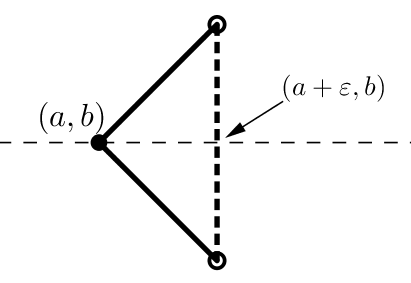
\includegraphics[scale = 1.5]{img/ExamenSeptiembre2017/Abiertosimg}
	\end{figure}
	Estos serán los abiertos de nuestra base de abiertos de la topología $\T$.
	Algo muy importante y que se resaltará siempre es que solo hemos de responder a lo que se nos pide. En este caso ya se nos dice que es una base de la topología, por lo tanto no tenemos que comprobarlo ni nada por el estilo. Podemos jugar con este hecho desde el principio, ya que nos lo da el enunciado.
	\begin{enumerate}
		\item Vamos a hacer una serie de apreciaciones antes de proceder a la resolución de este apartado. Hemos de observar que $\T_u \varsubsetneq \T$. Esto implica que la topología $\T$ es más fina que la usual. Esto se desprende de que cualquier abierto de de la usual contiene un abierto de $\T$, y que esta contención es estricta de que los triángulos no son abiertos en la usual.(La otra contención no se da ya que no podemos meter abiertos de la usual para ciertos puntos del triángulo, como por ejemplo el vértice).
		
		Vamos a calcular entonces la adherencia de un triángulo semiabierto. L aprimera idea intuitiva que nos surge es añadirle al abierto el segmento vertical con los extremos incluidos que une los dos vértices del triángulo.
		
		\begin{figure}[h!]
			\centering
			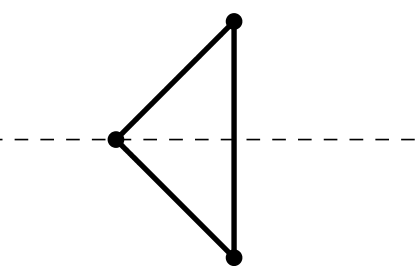
\includegraphics[scale = 1.5]{img/ExamenSeptiembre2017/Abiertosadherencia1img}
		\end{figure}
	
		Estos son cerrados en la topología usual, $\implies$ $\U \subset \adher{U}^{usual}$, luego  $\U \subset \adher{U}^{usual} \subset \adher{U}$.
		Ahora vamos a ver si los puntos que hemos añadido son adherentes. A esto respondemos que no (si llamamos $r$ al segmento citado), ya que $\forall p \in r , \exists V$ entorno de $p \tq \V \cap \U = \emptyset$.
		
		\begin{figure}[h!]
			\centering
			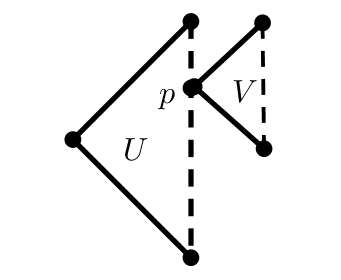
\includegraphics[scale = 1.5]{img/ExamenSeptiembre2017/Abiertosadherencia2img}
		\end{figure}
		
		Por lo tanto la adherencia de $\U$ en esta topología es el propio $\U$, ya que como hemos visto, los puntos de ese segmento no son adherentes.
		
		Si lo hubieramos visto comprobando ``uno a uno" todos los puntos habría que decir además que los puntos de fuera del triángulo no son adherentes ya que existe un abierto en la usual wque contiene un triángulo (que es entorno que no corta al conjunto).
		
		Luego  $\adher{\U} = \U$ , lo quer implica además que es una base de abiertos y cerrados simultaneamente.
		
		\item Veamos si el espacio topológico es Lindelöf con esta topología.
	\end{enumerate}	
\end{proof}